\section{Cubical Type Theory}

HoTT fails to achieve desirable computational behaviour.
In particular, Univalence is an axiom and Canonicity is not guaranteed for HITs.
HoTT affords presheaf model in simplicial sets.  
A computational model of type theory is then motivated using cubical sets in place for simplicial sets. 

\subsection{Cubical Sets}
Let there be a fixed disrete and countable set of \emph{names} $\A$ and define the set of \emph{directions} $\2 = \{0,1\}$.
\begin{definition}[The cubical category $\cube$][Coq]
  The cubical category $\cube$ has as objects finite subsets $I, J, K... \subseteq \A$.
  A morphism $f : I \to J$ is a set function $f : I \to J \cup \2$, such that 
  $f x = f y$ implies $x = y$ for $x,y \notin \2$. 
  The composition of morphisms $f : I \to J$ and $g : J \to K$ is defined as 
    $g \circ f (x) = g(f(x))$ when $f x \notin \2$ and $f x$ otherwise.
  
\end{definition}
We will call morphisms \emph{substitutions} as they encode sending a name to a direction.
We will also denote $fg$ for $g \circ f$ as well as $xf$ for $f(x)$ from now on (called diagram order),
and often omit braces in $I \cup \{x, y\}$ or $I - \{x,y\}$ for finite sets of names.

For $I \subseteq J$, we call the inclusion $f : I \to J$ a \emph{degeneracy map}. 
We have the \emph{face maps} $(x = 0), (x = 1) : I  \to I - x$ sending $x$ to $0$ and $1$ respectively. (Note how these constructions parallel the simplex category ${\Delta})$
\begin{definition}[Cubical sets]
  A cubical set $X$ is a covariant functor $X : \cube \to \Set$, i.e., a presheaf over $\cube^{op}$.
\end{definition}
That is, a cubical set $X$ is a collection of sets $X(I)$ and for any substitution $f : I \to J$, set functions $X(I) \to X(J)$, $u \mapsto uf$ such that $u\1 = u$ and $u(fg) = (uf)g$.
This can be thought of as $X(\varnothing)$ is the set of points of a space, $X(x)$ are its lines, $X(x,y)$ are squares, and so on.
\[
\begin{tikzcd}[row sep=large, column sep=large]
u(0,1) \arrow[r, "u(y=1)"] & u(1,1)\\
u(0,0) \arrow[u, "u(x=0)"] \arrow[r, "u(y=0)"']  & u(1,0) \arrow[u, "u(x=1)"']
\end{tikzcd}
\quad
\begin{tikzpicture}[baseline={(0,0)}]
  \draw[->] (0,0) -- (0.5,0) node[right] {$x$};
  \draw[->] (0,0) -- (0,0.5) node[above] {$y$};
\end{tikzpicture}
\]

Cubical sets form a presheaf category, i.e. $\cSet := [\square, \Set]$ with morphisms given by 
natural transformations.
\begin{example}
  Let $A$ be a set. Then $X : \cube \to \Set$ with $X(\varnothing) = A$ and $X(I) = \varnothing$ if $I \neq \varnothing$
  is called the discrete cubical set over $A$.
\end{example}
\begin{example}
  Let $R$ be a commutative ring. Then $R[\cdot]$ is a cubical set, with $R[I]$ being the polynomial ring over $I$,
  and for $f : I \to J$, $R[f](x) = f(x)$ where $0$ and $1$ in $\2$ are swapped for $0$ and $1$ from $R$. 
\end{example}

\begin{example}[Interval] 
  The interval $\I$ is the cubical set defined by $\I(I) = I \cup \2$ and for $f : I \to J$,
  $\I(f)$ is the extension of the set theoretic map of $f$ such that $\I(f)(0) = 0$
  and $\I(f)(1) = 1$.
\end{example}

Note that for a fixed name $x$, $\I \cong \mathbf{y}\{x\}$, where $\mathbf{y}$ is the Yoneda embedding.
More generally, $\cube_I = \mathbf{y}I$ where $I$ contains $n$ elements, is the representable $n$-cube (since $\mathbf{y}I \cong \mathbf{y}J$ for $I \cong J$).

\begin{definition}[Non-dependent Path Space]  
  Given a cubical set $X$, we define its \emph{path space} $[\I]X$ as a cubical set $([\I]X)(I) = X(I,x_I)$ where $x_I$ is a fresh name $(x_I) \notin I$.
  Let $f : I \to J$ be a sustitution, then $X(f)$ is given by the induced map from $f$ via inclusion, composed with substituting $x_I$ for $x_J$, i.e.,
  $\omega (X(f))= \omega f(x_I = x_J)$.
\end{definition}
For a cubical set $X$, $[\I]X$ is also a cubical set. $[\I]X(\varnothing)$ are the points, $[\I]X(x)$ are the lines, $[\I]X(x,y)$ are the squares,
and so on.

\begin{definition}[Non-dependent Identity Type]
  Given a cubical set $X$, and $a, b \in X(\varnothing)$, the \emph{identity type} $\Id_X(a,b)$ is the subobject of $[\I]X$ such that
  $\omega \in (\Id_X(a,b))(I)$ iff there is some name $x \in I$ such that $\omega(x =  0) = a$ and $\omega(x = 1) = b$. 
\end{definition}

\subsection{The Uniform Kan Condition}

\begin{definition}[Open boxes] 
  Let $X$ be a cubical set. Let $I$ be a finite set of names, and $x, J \subseteq I$, with $x \notin J$.
  Fix $a$ either $0$ or $1$.
  An \emph{open box} denoted $\vec{u}$ is a family of faces $u_{yb}$ in $X(I - y)$ for each $(y,b)$ either $(x,a)$ or $y \in J, b = 0,1$.
  such that \[u_{yb} (z = a) = u_{za}(y = b)\] for all $y, z \in J, y \neq z$ and $b, c = 0, 1$.
\end{definition}
The idea is that an open box contains all faces, except for one face in a direction $x$.

\begin{definition}[Kan Cubical Set]
  A Kan cubical set $X$ is a cubical set $X$, equipped with \emph{filling operations} $X\fillup$, and $X\filldown$,
  such that for every $J,x \in I$, $X\fillup \vec{u}, X \filldown \vec{u}$ are in $X(I)$, where $\vec{u}$ is an open box
  with $u_{x0}$ and $u_{x1}$ in $X(I - x)$ in the respective cases $X \fillup \vec{u}$ and $X \filldown \vec{u}$, such that the following condition holds:
  \[
    (X \fillup \vec{u})(y = b) = u_{yb} \text{ \emph{and} } (X \filldown \vec{u})(x = b) = u_{yb}
  \]
  along with the `uniformity/coherence' condition, that for $f : I \to K$ defined on $J,x$, we require:
  \[
    (X \fillup \vec{u}) f = X \fillup (\vec{u} f) \text{\emph{ and }} (X \filldown \vec{u}) = X \filldown (\vec{u} f) \]
\end{definition}
We also denote $X^{+} \vec{u} = X \fillup \vec{u} (x = 1)$ and $X^{-} \vec{u} = X \filldown \vec{u} (x = 0)$.
This condition for $X$, known as the \emph{Kan condition} is the analogous statement to \emph{``every horn has a filler"} for Kan complexes, i.e., \emph{``every open box has a filler"}.
\[
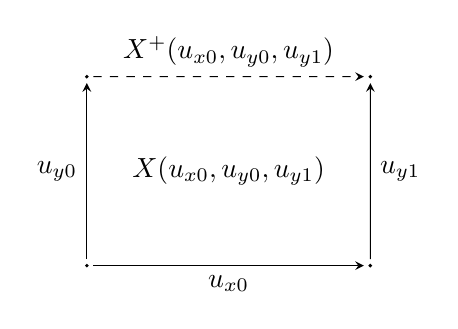
\begin{tikzpicture}[scale=1.2, >=stealth]
  \node[circle, fill, inner sep=0.5pt] (A) at (0,0) {};
  \node[circle, fill, inner sep=0.5pt] (B) at (3,0) {};
  \node[circle, fill, inner sep=0.5pt] (C) at (0,2) {};
  \node[circle, fill, inner sep=0.5pt] (D) at (3,2) {};


  % Corner nodes (filled dots)
  \node[circle, inner sep=1.5pt] (A) at (0,0) {};
  \node[circle, inner sep=1.5pt] (B) at (3,0) {};
  \node[circle, inner sep=1.5pt] (C) at (0,2) {};
  \node[circle, inner sep=1.5pt] (D) at (3,2) {};

  % Edges (arrows automatically stop at node boundary)
  \draw[->] (A) -- node[below] {$u_{x0}$} (B);
  \draw[->] (A) -- node[left] {$u_{y0}$} (C);
  \draw[->] (B) -- node[right] {$u_{y1}$} (D);

  % Dashed top edge
  \draw[->, dashed] (C) -- node[above] {$X^{+} (u_{x0},u_{y0},u_{y1})$} (D);

  % Interior label
  \node at (1.5,1) {$X \fillup (u_{x0},u_{y0},u_{y1})$};

\end{tikzpicture}
\]

Any presheaf category gives rise to a model of dependent type theory by intepreting each presheaf as a type.~\cite{hofmann97} 
Hence, cubical sets form such a model with (dependent) products, (dependent) sums, inductive types and identity types.
We refine this model by restricting to Kan Cubical Sets taken along with a specified `Kan Structure',
which are the Kan filling operations $X \fillup$ and $X \filldown$. This is needed in order to justify the elimination rules for identity types.~\cite{bezem2014model}
Consequently, we can prove functional extentionality, univalence, canonicity for HITs.
For a complete, formal treatment, see Simon Huber's PhD Thesis for more details.~\cite{huberphd}


